\section{Ignitions}
\pgfdeclareimage[width=1.0\paperwidth]{header-image}{header_images/red_lightn}

\begin{frame}
    \frametitle{Igntions}
    \framesubtitle{Humans and Natural $<$ Humans + Natural}

	\begin{textblock*}{11cm}(0cm,2cm)
    \begin{tikzpicture}
        \visible<1->{
        	\node[anchor=south west,inner sep=0] (image) at (0,0) {
	            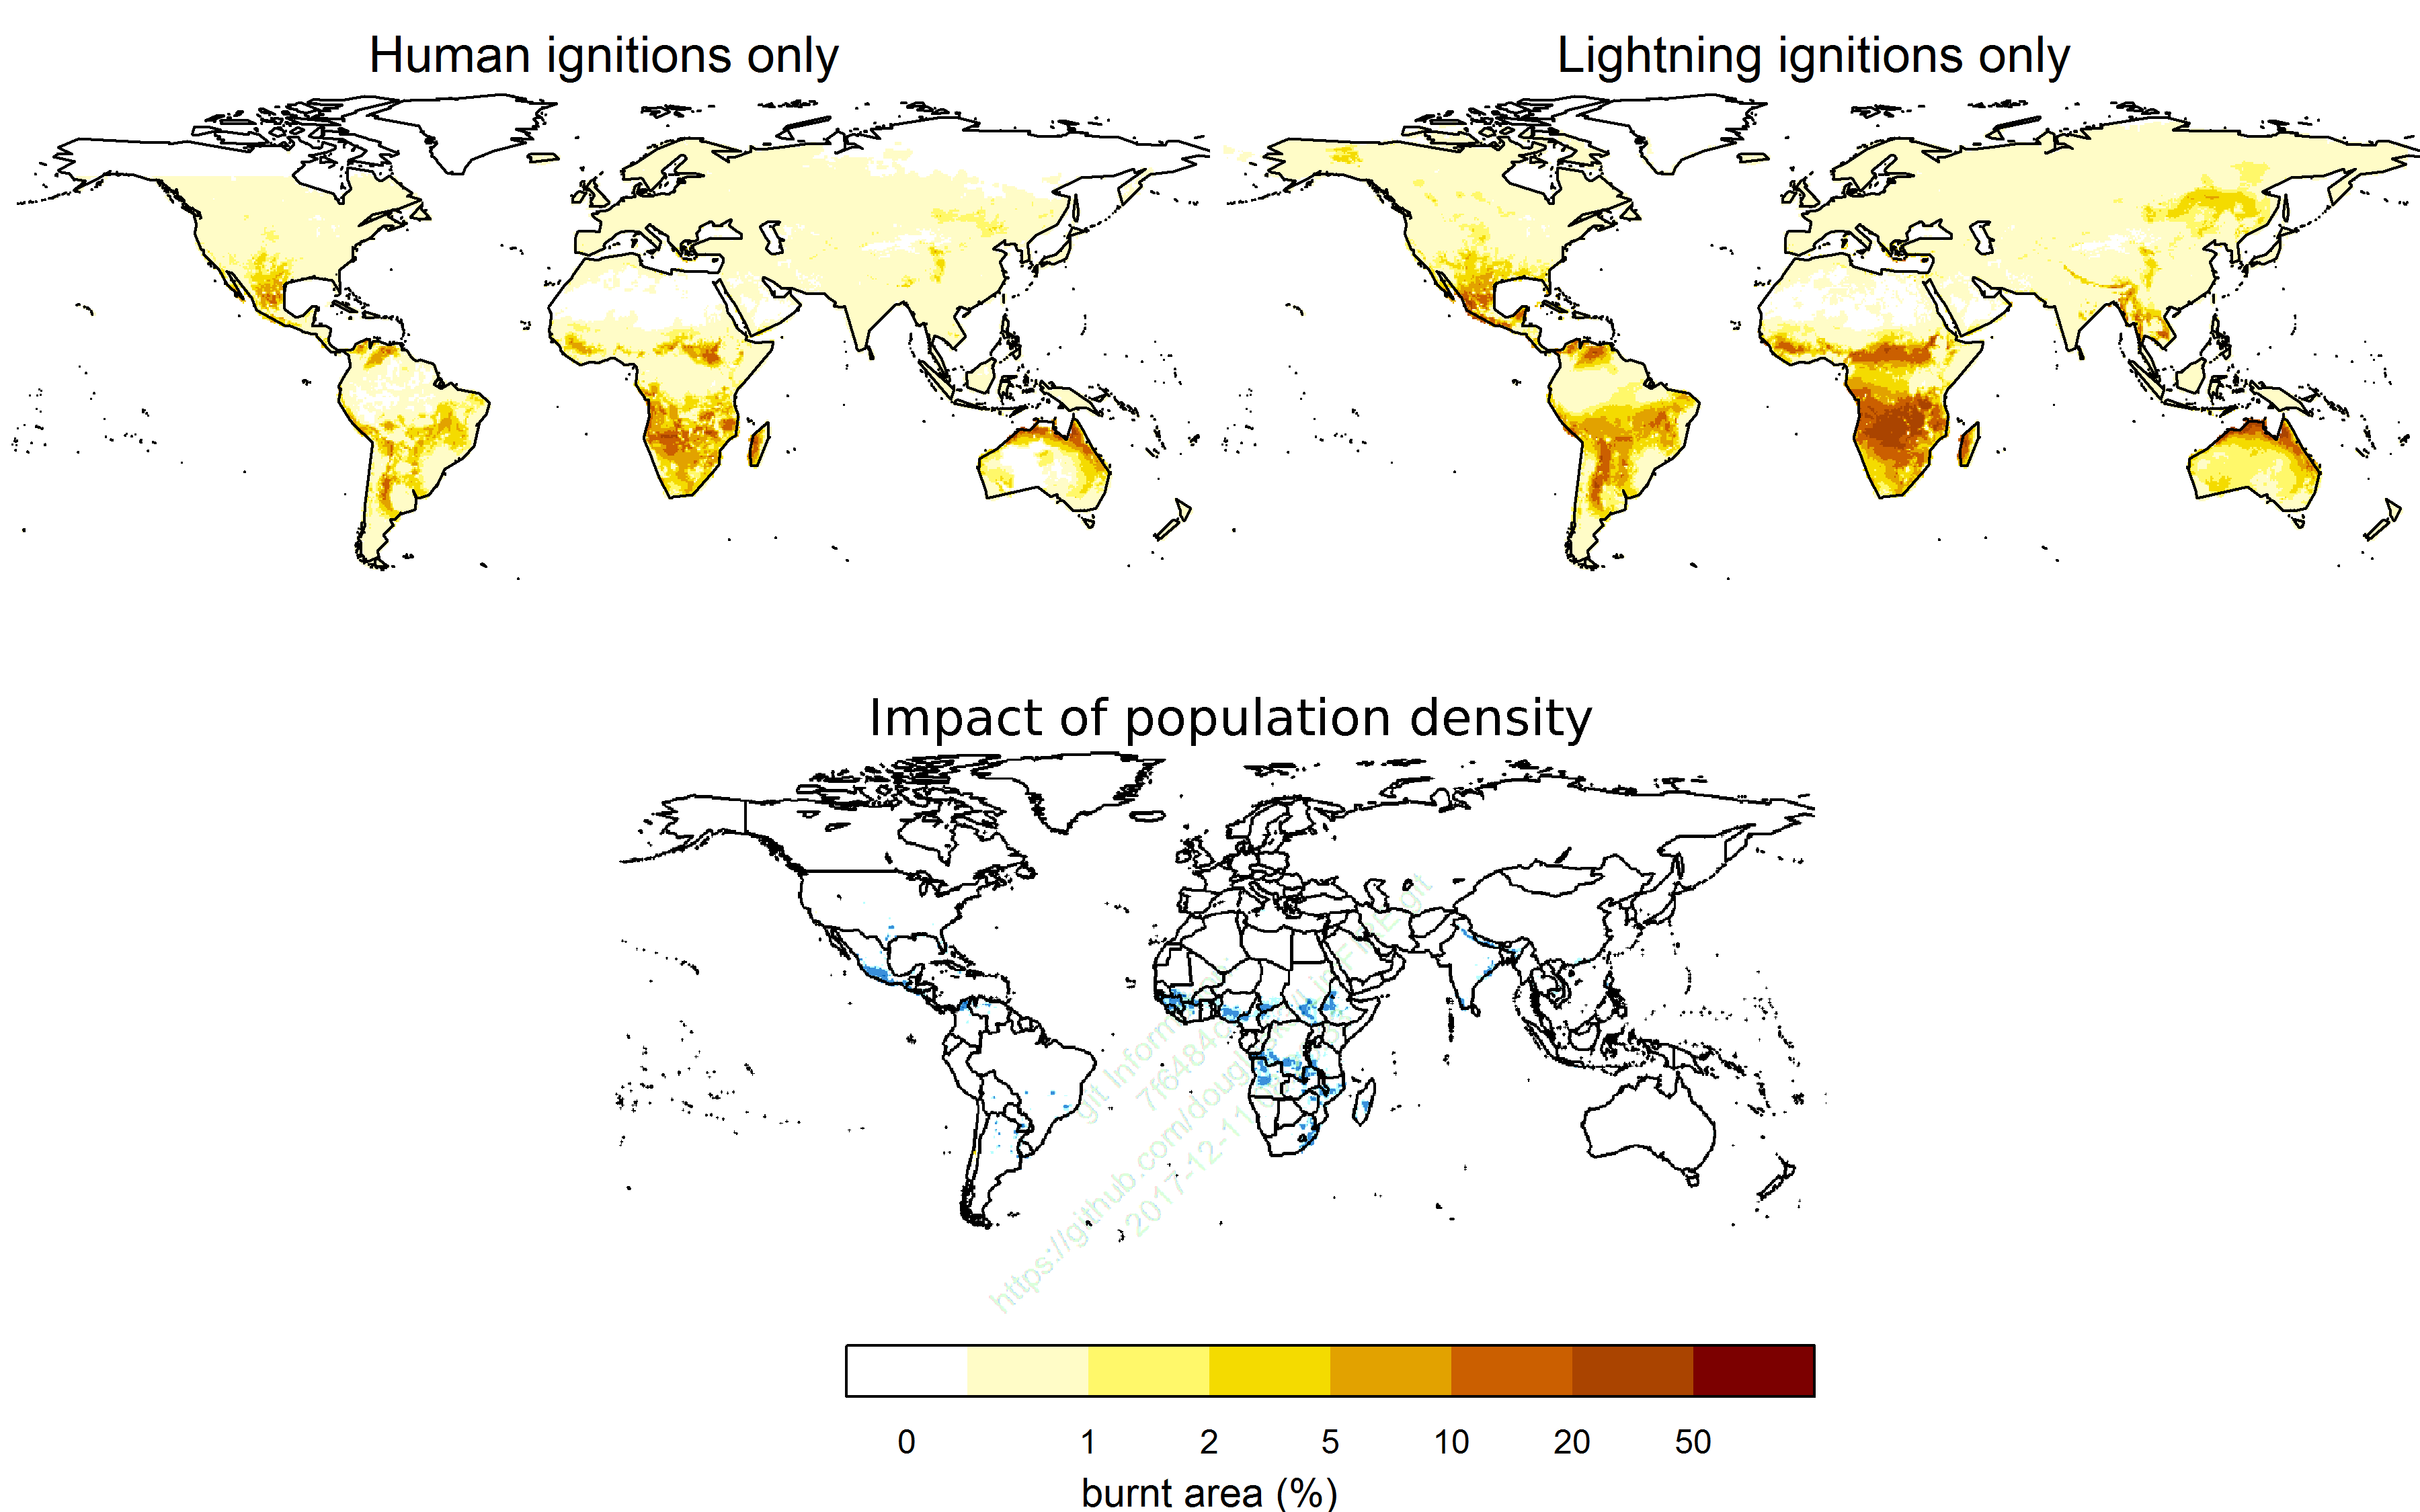
\includegraphics[trim={0cm 10cm 10cm 0cm},clip, width=6.0cm]
		            {images/igntitions/IgntionInfoSourceAdding}
        };}

    %\end{tikzpicture}
    %\end{textblock*}
	%\begin{textblock*}{6cm}(0cm,2cm)
		%\begin{tikzpicture}
		\visible<2->{
			\node[anchor=south west,inner sep=0] (image) at (3,-2) {
				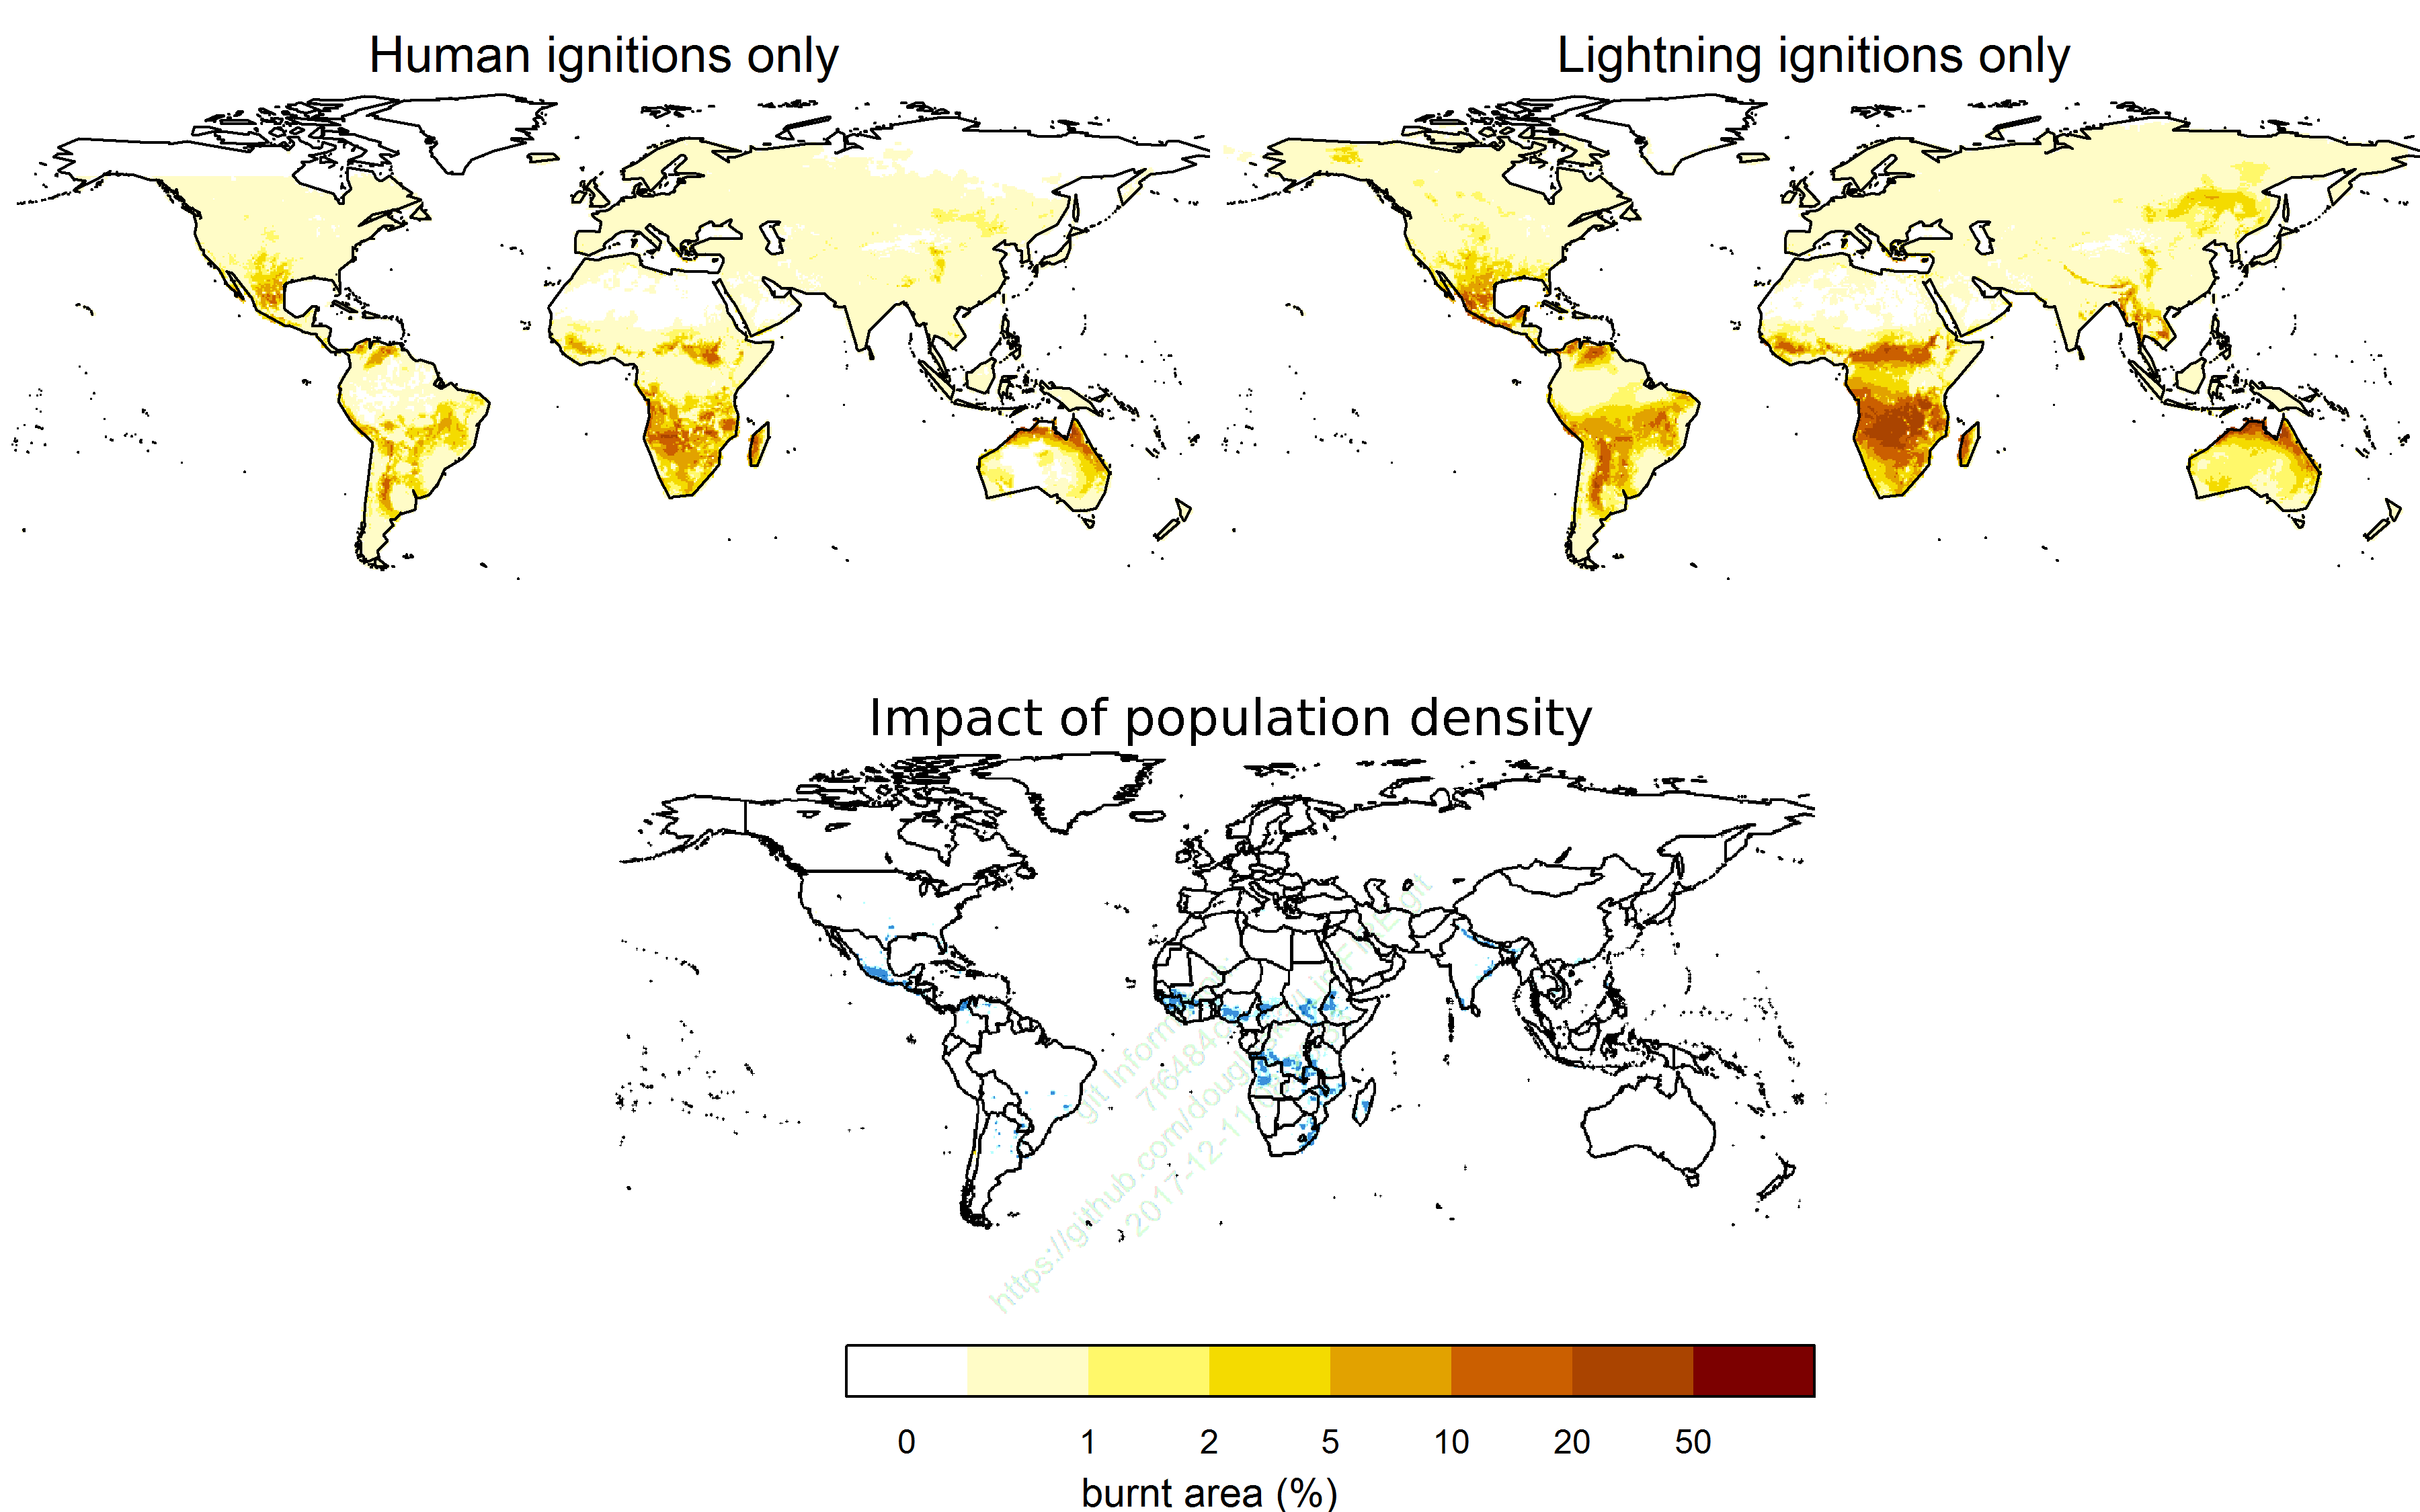
\includegraphics[trim={10cm 10cm 0cm 0cm},clip, width=6.0cm]
				{images/igntitions/IgntionInfoSourceAdding}
			};}
		\visible<3->{
			\node[anchor=south west,inner sep=0] (image) at (8,-6) {
				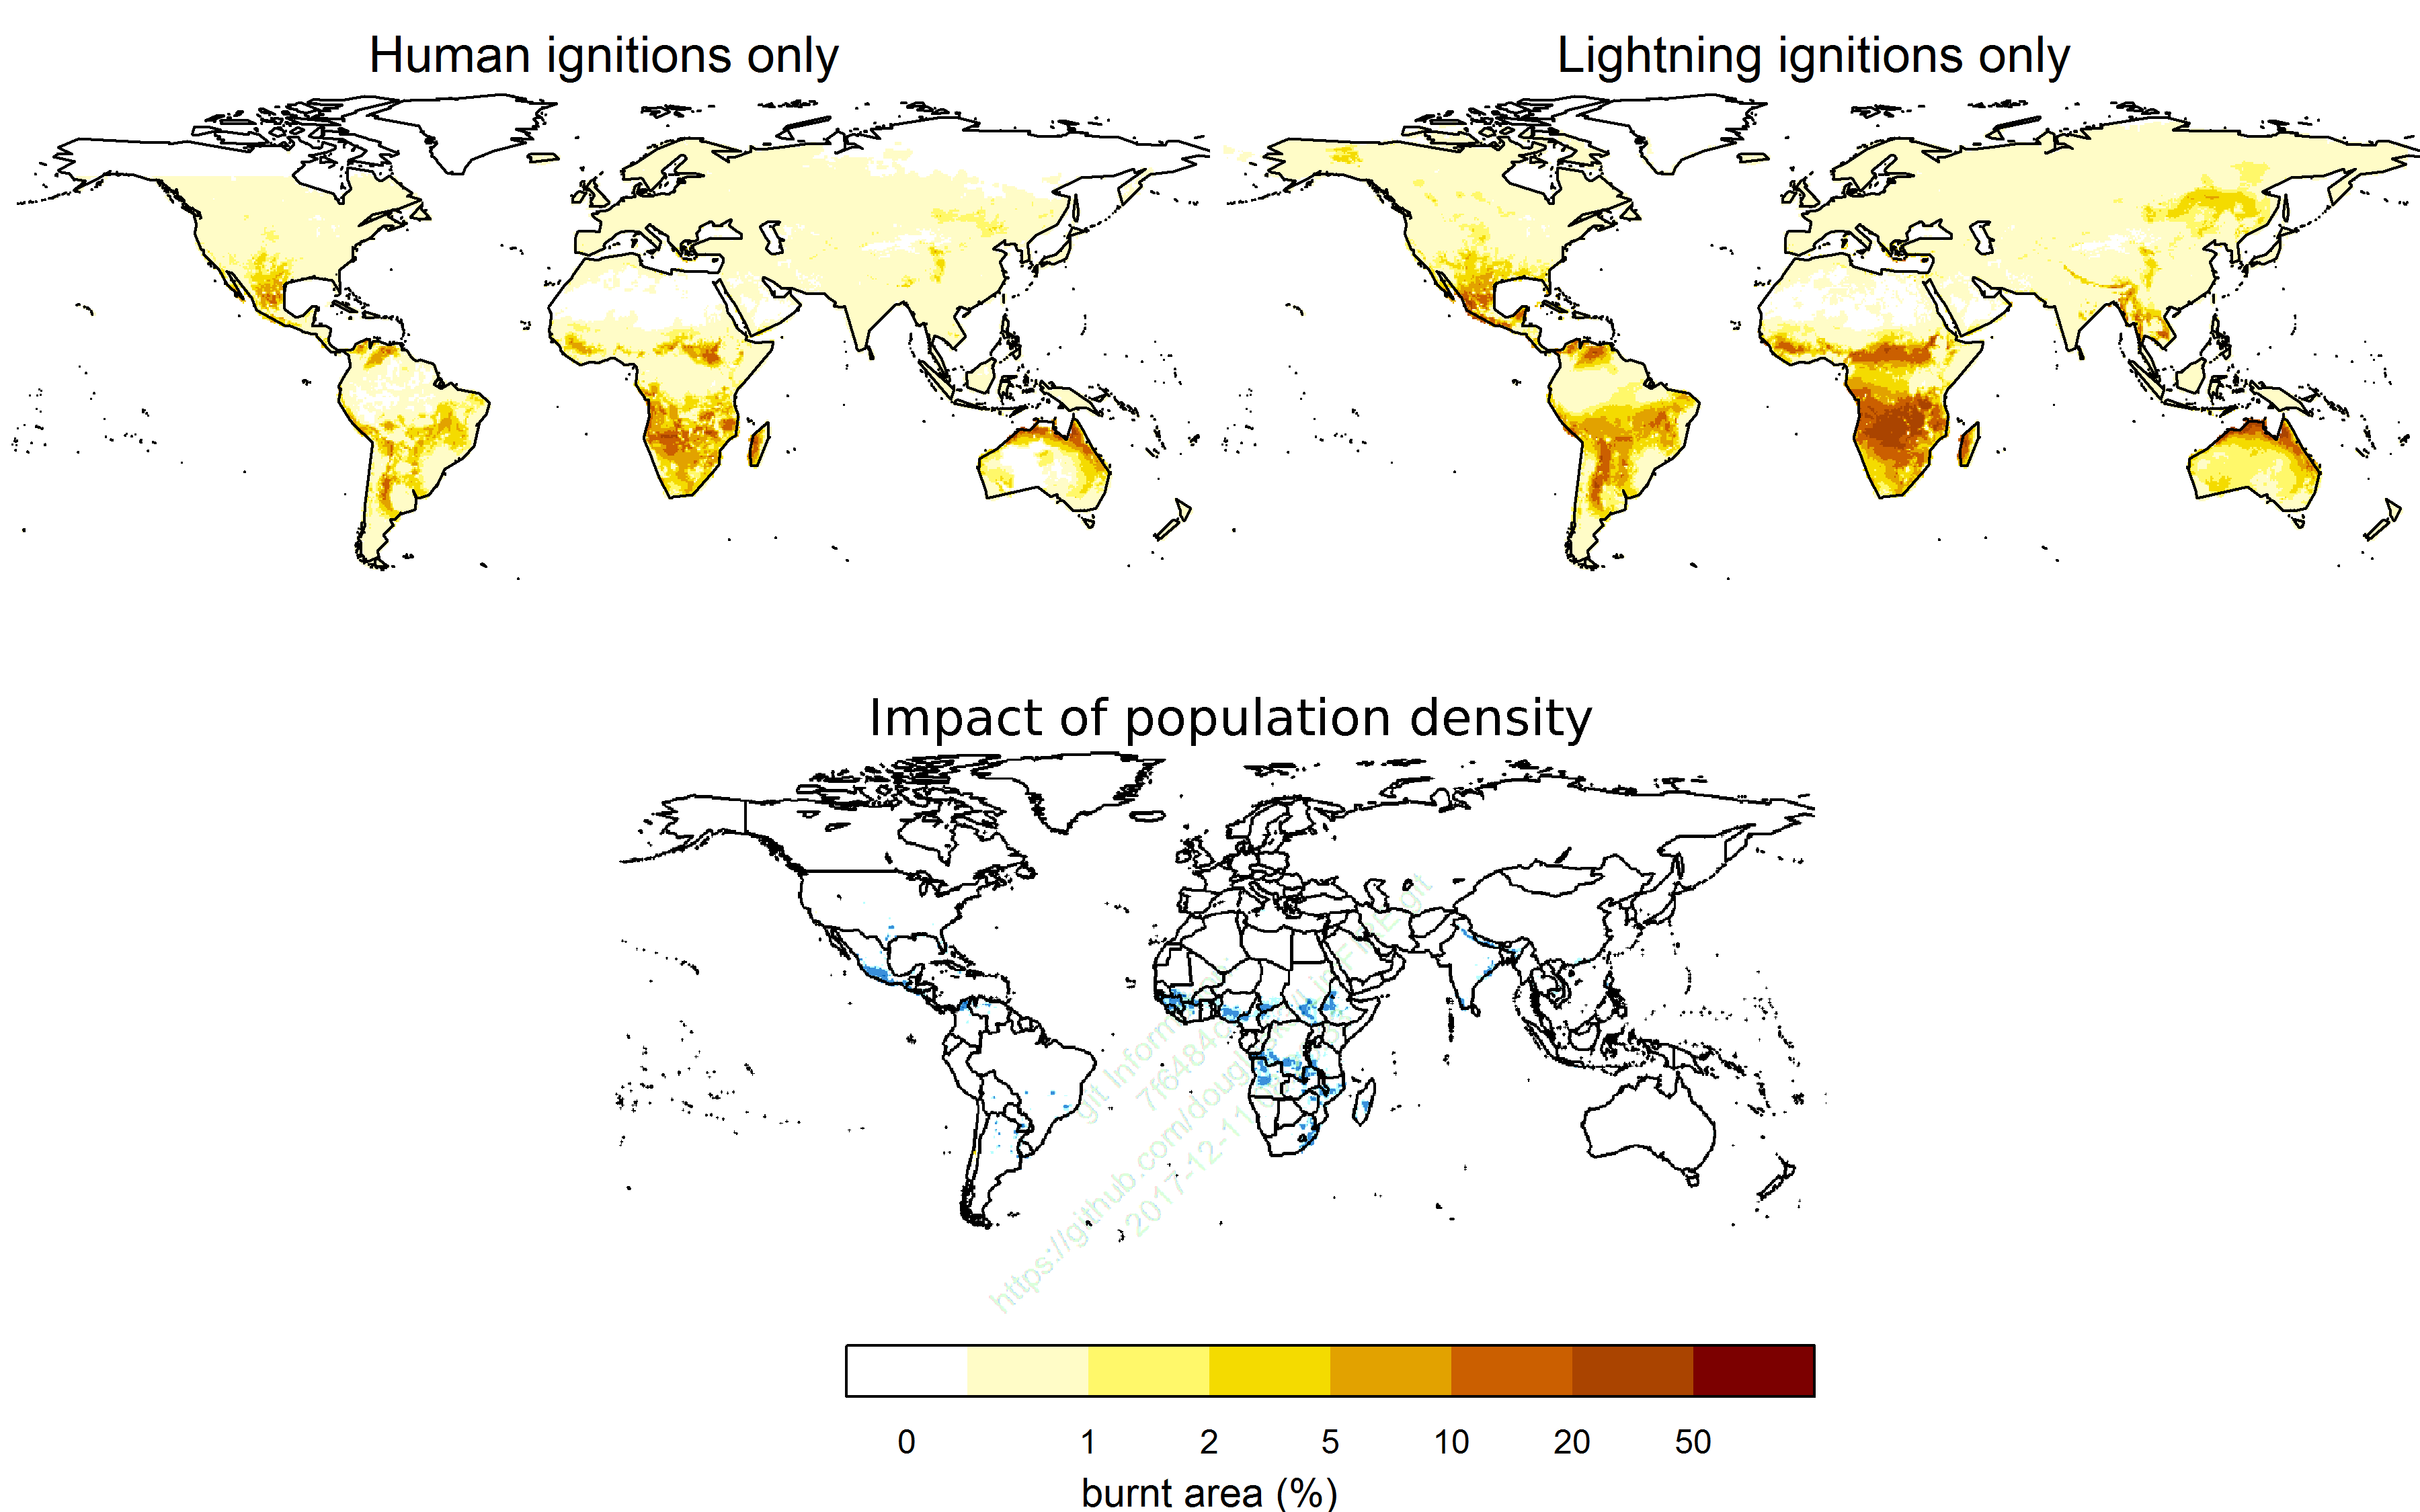
\includegraphics[trim={10cm 0cm 0cm 5cm},clip, width=6.0cm]
				{images/igntitions/IgntionInfoSourceAdding}
			};}
		
		\end{tikzpicture}
	\end{textblock*}
	%trim = {l b r t}
\end{frame}

\begin{frame}
    \frametitle{Ignitions}
    \framesubtitle{Which is more important}
    %\node[anchor=south west,inner sep=0] (image) at (0,0) {
    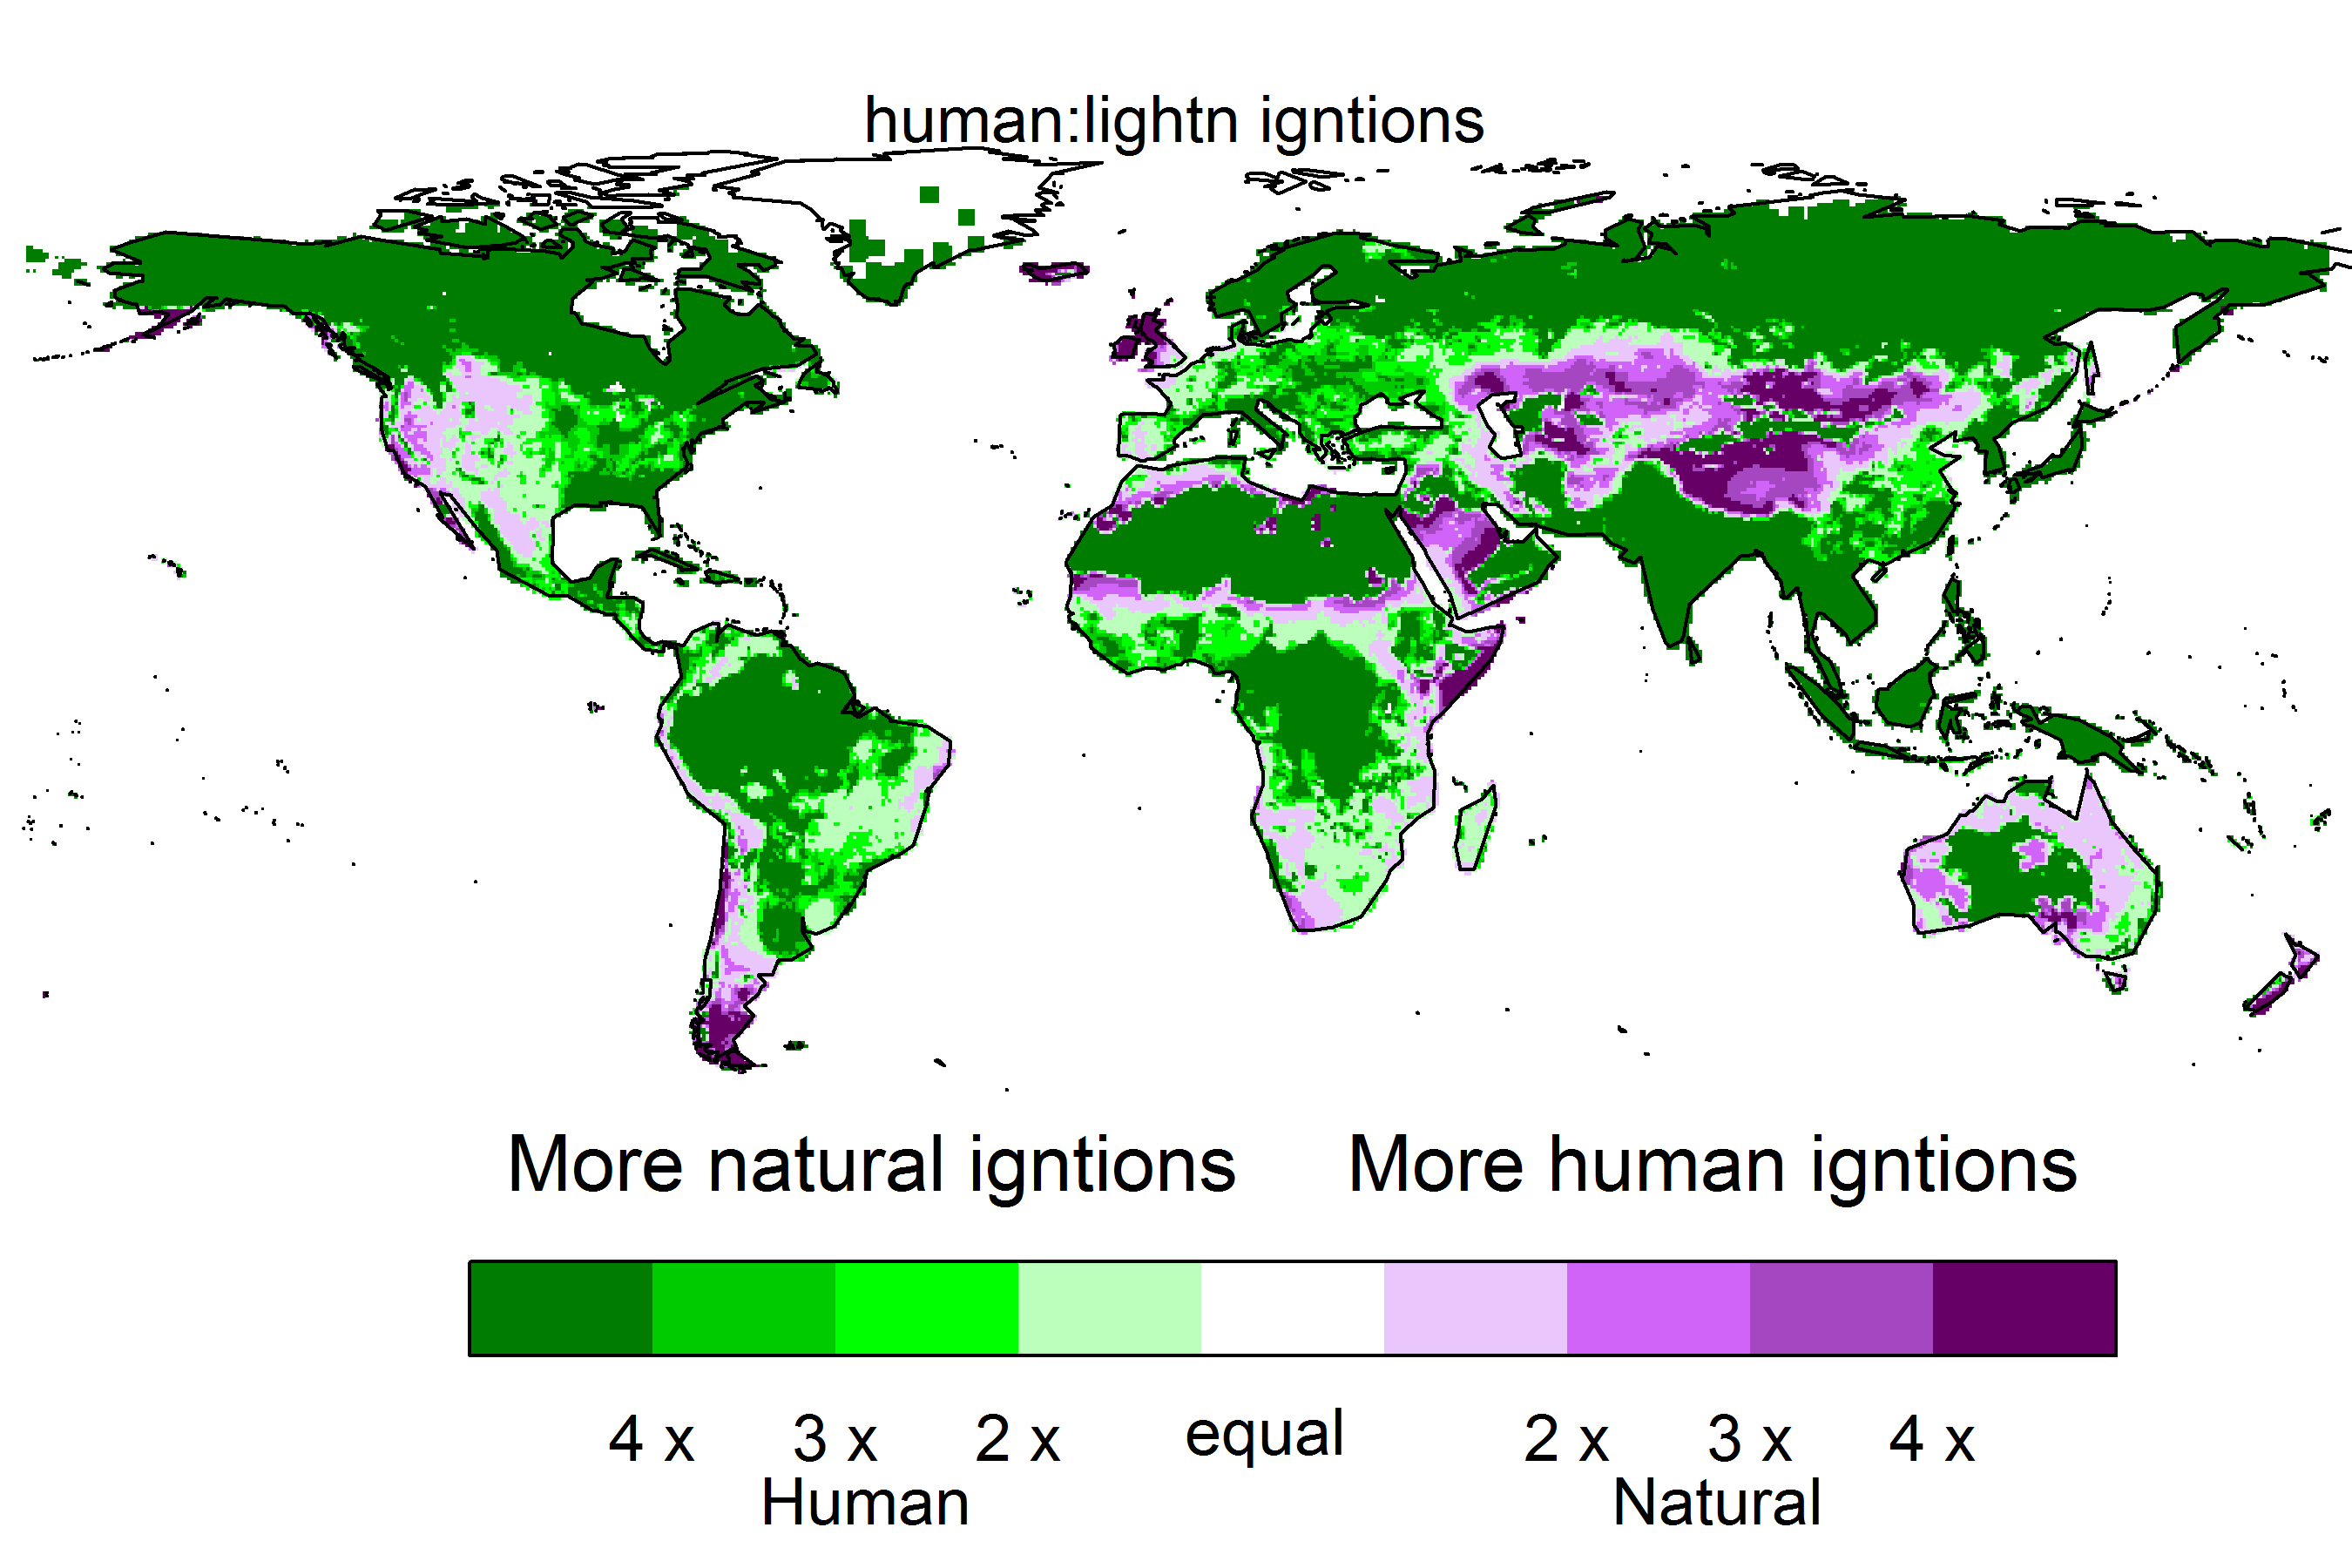
\includegraphics[width=11.0cm]{images/igntitions/IgntionInfosourceImportance}

\end{frame}

%\begin{frame}
%    \frametitle{Igntions}
%    \framesubtitle{Igntion saturattion and manipulation}
%\end{frame}
